%% LaTeX2e class for student theses
%% sections/evaluation.tex
%% 
%% Karlsruhe Institute of Technology
%% Institute for Program Structures and Data Organization
%% Chair for Software Design and Quality (SDQ)
%%
%% Dr.-Ing. Erik Burger
%% burger@kit.edu
%%
%% Version 1.2, 2016-09-20

\chapter{Data Transmission Experiments}
\label{ch:Evaluation}

The final proof-of-principle to demonstrate the functionality of a multi-chip module is the realization of a real data transmission experiment that uses the built MCM as the data source, and is received by an optical receiver that demodulates and interprets the information carried in the lightwave in a communication link. The receiver used are characterized, unamplified photodiode modules that decouple the receiver behavior from the transmitter performance, such that the latter can be assessed through the results of the data transmission experiment.
\par\medskip
In this chapter, the details of the implementations used throughout the data transmission experiments procedure are discussed and reviewed. The description of the demonstrators featuring direct detection (MZM modulator) and coherent detection (IQ modulator) are presented, including the setup used for each case and the discussion of the results obtained. All measurements were done with PWB with air as an overcladding.

%\textbf{Data transmission experiment}: The final step to corroborate the performance of the multi-chip module requires the device to be tested  transmitting sample data in order to characterize its transmission properties. The bit error probability (BER) is the most significant figure of merit, along with the external testing conditions (use of erbium-doped fiber amplifier (EDFA); use of gate voltage; use of attenuators, etc.) used to reach such quantity.

\section{Direct Detection Data Transmission Experiment}

\begin{figure}[!ht]
\centering
  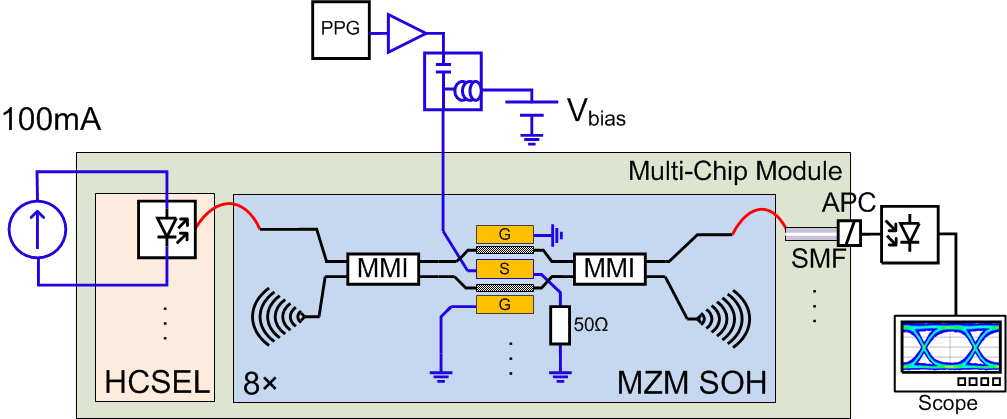
\includegraphics[width=0.8\textwidth]{visio/MCM-LO_DTE}
  \caption{Initial MCM direct detection data transmission experiment. The HCSEL is powered by a precision current source set at \SI{100}{\milli\ampere}. For data injection, a pulse pattern generator (PPG) with an RF amplifier  is connected to the MZM signal probe, terminated with a \SI{50}{\ohm} external resistor. The launched light is connected through an angled connector to the photoreceiver and analyzed with a scope.}
  \label{fig:mcm-001-DTE}
\end{figure}

The components used in the direct detection data transmission experiment setup are schematically represented in figure \ref{fig:mcm-001-DTE}. A high-precision external current source is set to \SI{100}{\milli\ampere} to provide power for the HCSEL. The MZM signal terminal is impedance-matched with a \SI{50}{\ohm} termination resistor, and a programmable pattern generator (PPG) with an RF amplifier is used as a signal source to modulate the MZM, coupled to the circuit with a bias tee and an independent external voltage source. The modulated signal is sent through a single mode fiber (SMF) with an angled connector (APC) to a photodiode receiver into a scope to analyze the corresponding received signal. The eye diagram mask is shown in figure \ref{fig:MCM1}. The calculated BER is obtained as in appendix \ref{sec:appendix:calcBER}, yielding a value of \SI{2.2e-3}. %In this case, \SI{10}{\giga bit/\second}, and no EDFA or gate voltage is applied. The signal obtained is only the electrical eye diagram. 

\begin{figure}[!ht]
\centering
  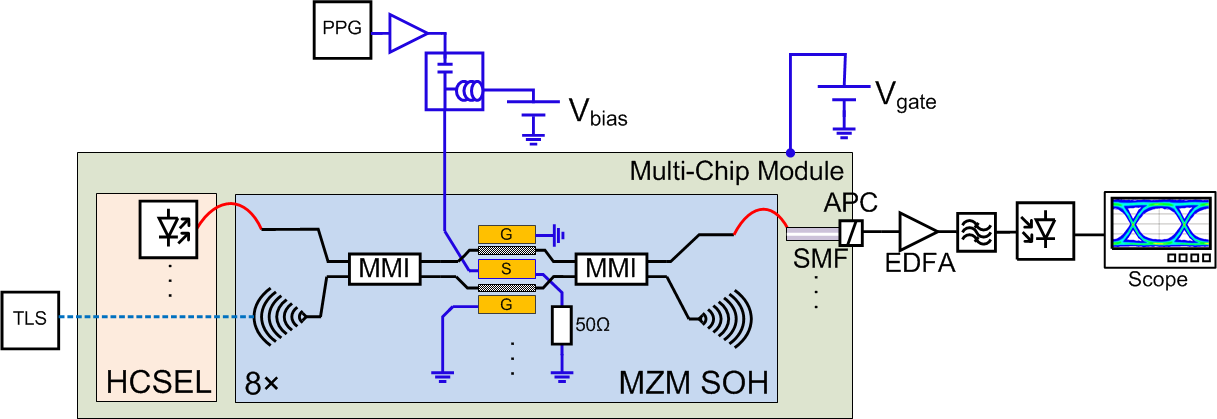
\includegraphics[width=0.8\textwidth]{visio/MCM-LO_DTE_GV}
  \caption{First MCM data transmission experiment with gate voltage implemented diagram. Light is injected to the MZM through an external tunable laser source (TLS). For data injection, a pulse pattern generator is connected to an RF amplifier and a bias tee through a GSG picoprobe. The MZM is terminated with a \SI {50}{\ohm} external resistor. The outcoupled light is detected by a photoreceiver connected to a vector signal analyzer (VSA). Gate voltage (inside a dashed line) was added later in the process.}
  \label{fig:mcm-001-DTE-GV}
\end{figure}


\begin{figure}[!ht]
\centering
\begin{tabular}{cc}
\subfloat[\SI{10}{\giga bit/\second},$V_\text{gate}=\SI{0}{}$, no EDFA]{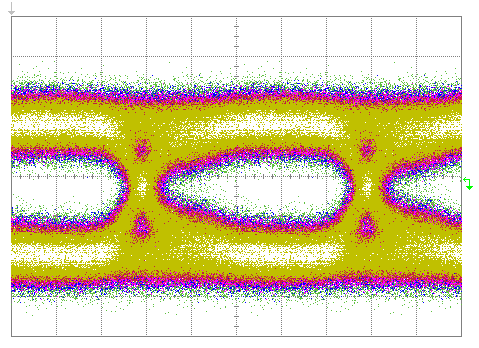
\includegraphics[width=0.45\textwidth]{caps/opt_10G_gate50V_noedfa}\label{fig:MCM1}} &
%\subfloat[E, \SI{40}{\giga bit/\second},$V_\text{gate}=\SI{50}{\volt}$, with EDFA]{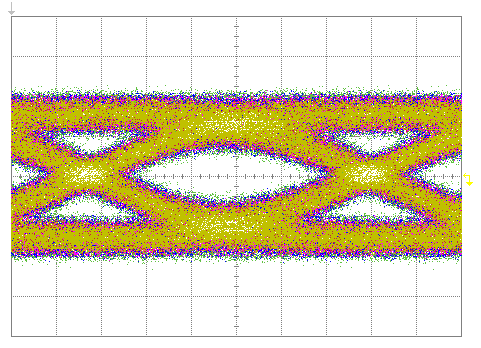
\includegraphics[width=0.45\textwidth]{caps/el_40G_gate50V_edfa}\label{fig:MCM2}} \\
\subfloat[\SI{40}{\giga bit/\second},$V_\text{gate}=\SI{50}{\volt}$, with EDFA]{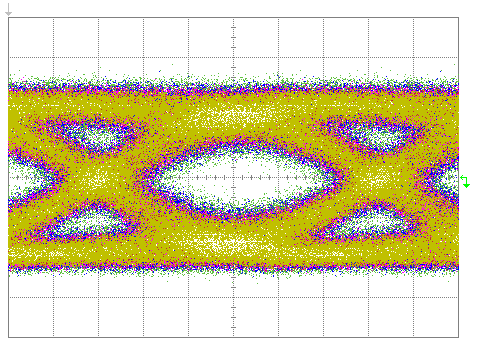
\includegraphics[width=0.45\textwidth]{caps/opt_40G_gate50V_edfa}\label{fig:MCM3}} %&
%\subfloat[O, \SI{10}{\giga bit/\second},$V_\text{gate}=\SI{100}{\volt}$, with EDFA]{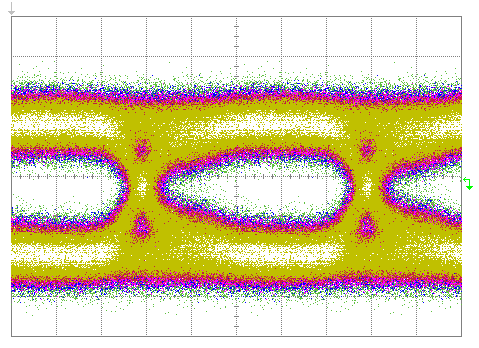
\includegraphics[width=0.45\textwidth]{caps/opt_10G_gate50V_noedfa}\label{fig:MCM4}} 
\end{tabular}
\caption{MCM direct detection eye diagrams; Data rate for each case are noted, as well as the applied gate voltage and whether an EDFA was used for optical amplification.}
\label{fig:MCM_gateEDFA}
\end{figure}
%\begin{figure}[!ht]
%\centering
%  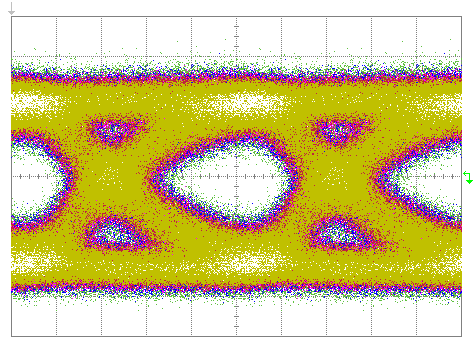
\includegraphics[width=0.8\textwidth]{caps/SOH_10G_E_NOG}
%  \caption{MCM eye diagram at \SI{10}{\giga bit/\second}, \SI{20}{\pico\second/div}.}
%  \label{fig:mcm-001-eye1}
%\end{figure}

%\lasnotas{which is driven to depletion, and thus no free carrier absorption occurs,  and thus a slot waveguide lying on top of an insulating layer (in the specific case of this thesis, \ce{SiO2}) will present band bending due to majority carrier accumulation. MAYBE PUT THIS SOMEWHERE ELSE}.  The MCM was tested at \SI{40}{\giga bit/\second}, but no eye was visible under the aforementioned conditions. 
In order to further push the performance of the MCM, the addition of gate voltage and the use of an erbium-doped fiber amplifier (EDFA) was suggested and added to the setup. The schematic diagram of the setup is presented in figure \ref{fig:mcm-001-DTE-GV}. As explained in appendix \ref{sec:appendix:gatevolt}, a large positive voltage is applied to the silicon (\ce{Si}) substrate to allow inversion in the metal-semiconductor-isolator boundary and thus allowing for improved carrier concentration and mobility. The setup also changes to an external laser source (ECL), since there was a suspicion of possible damage to the HCSEL due to the ground of the first demonstrator MCM being tied together (due to the metallic aluminum substrate). The launch is done through the PWB through the APC connector and an EDFA with a filter is used to amplify the optical signal and analyzed with a scope.



Figure \ref{fig:MCM_gateEDFA} shows the most prominent results of the data transmission experiment using an MZM modulator. In figure \ref{fig:MCM1} the device is tested at low transmission speeds and measuring the optical eye mask. It can be seen that the eye rise time has a smaller slew rate than the falling edge causing duty-cycle jitter. This can be phenomenologically explained by the Mach-Zender modulator being slightly unbalanced, much like its analog effect in RF electrical circuits, referred to as common mode noise \cite{DjordjevicCM10}. The effect can be translated to optical fields due to an inhomogeneous field distribution where the gate voltage is applied. The effect was reviewed in super-junction LDMOS (laterally-diffused metal-oxide semiconductors) in an SOI substrate by Wang \cite{WangGV09}, where charge imbalance in the junction requiring tuning of the charges in the semiconductor junction regions. Since the structure of the MZM also has different electric field interactions in each arm, the results observed in the work of Wang. Figure \ref{fig:MCM3} show the case for gate voltage applied, for optical detection. The results reveal a promising result towards \SI{100}{\giga bit/\second} fully-functional performance, which was not tested because of the equipment limitation (the highest achievable data rate for direct detection is \SI{40}{\giga bit/\second} with the current settings). Finally, the data transmission experiment shows that there is no inherent data rate limitation on the SOH device.   %Finally, figure \ref{fig:MCM3}, shows an increased gate voltage test, which again shows duty-cycle jitter due to rise and fall time asymmetries.
%\FloatBarrier
%\clearpage

\section{Coherent Detection Data Transmission Experiment}

\begin{figure}[!ht]
\centering
  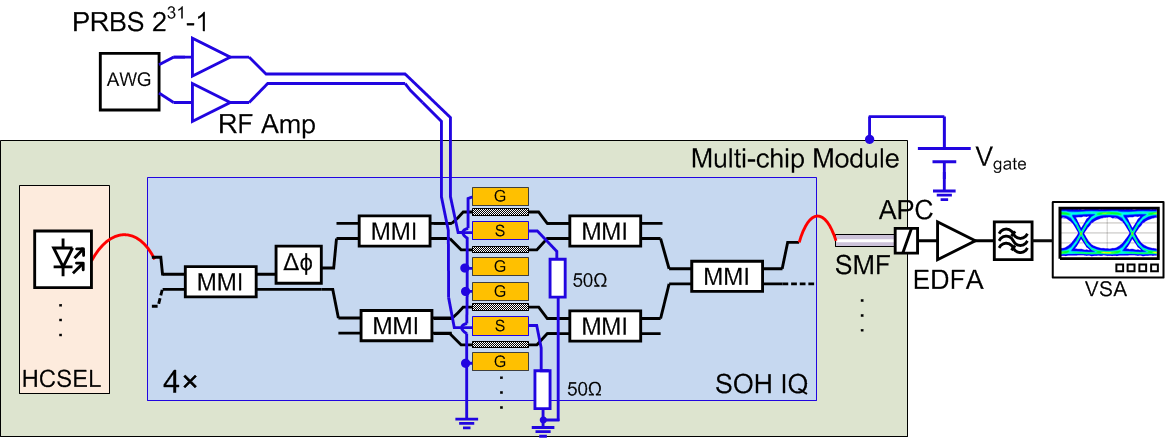
\includegraphics[width=0.8\textwidth]{visio/MCM-LO-IQ-DTE}
  \caption{MCM IQ data transmission experiment diagram. Light is coupled to the MZM through a PWB connected to a HCSEL, and externally modulated. An arbitrary waveform generator (AWG) with at least two channels is connected via an RF amplifier and a bias tee to each branch of the IQ modulator and terminated externally with \SI{50}{\ohm} resistors. Light is outcoupled to an EDFA, an passband filter and visualized through a VSA. Gate voltage is applied externally to the submount of the chip.}
  \label{fig:mcm-005-DTE-IQ}
\end{figure}

The next data transmission experiment was done after a homogeneous $V_\pi$ and transmission were obtained through processing iterations, and an IQ modulation was chosen because it proves the performance of the SOH platform, at the expense of more difficult fine tuning and a more complex setup, which is shown schematically in figure \ref{fig:mcm-005-DTE-IQ}. The data injection scheme is now done through an arbitrary wave generator (AWG) with 4 channels, connected through a bias tee using GSG microprobes on both sides of the MCM, and terminated with \SI{50}{\ohm} resistors for each modulator. A gate voltage $V_\text{gate}=\SI{100}{\volt}$ is applied to the module for its known improvement of the chip performance. The IQ modulators feature thermal phase shifters, consisting on resistive layers in the IQ modulator that can be modified through voltage, also controlled by an external DC source up to \SI{5}{\volt}. At the fiber output, an EDFA is connected to a bandpass filter and connected to an optical modulation analyzer (OMA) for visualization of the eye diagrams.

Each arm of the IQ modulator is independently optimized for best performance, and then calibrated for jitter and skew of both arms. Thermal shifters are used to obtain the optimum pre-compensation which was post-processed and applied to achieve the best possible transmission. Finally, a Kalman filter for phase tracking was implemented to overcome the considerable phase noise of the HCSEL. Another possible limitation was due to the relatively high $V_\pi$ of the SOH modulators. Nonetheless, it is low enough that non-linearities are observed in 16QAM modulation when using RF amplifiers. Figure \ref{fig:mcm-005-DTE-res} shows the summary of the measurements, with the best achievable speed being 16QAM, 56 Gbaud featuring a bit error probability (BER) of \SI{8e-3}{} and a forward error correction (FEC) of 20\%, with a total potential transmission data rate of 716 Gbit/s.

\begin{figure}[!ht]
\centering
  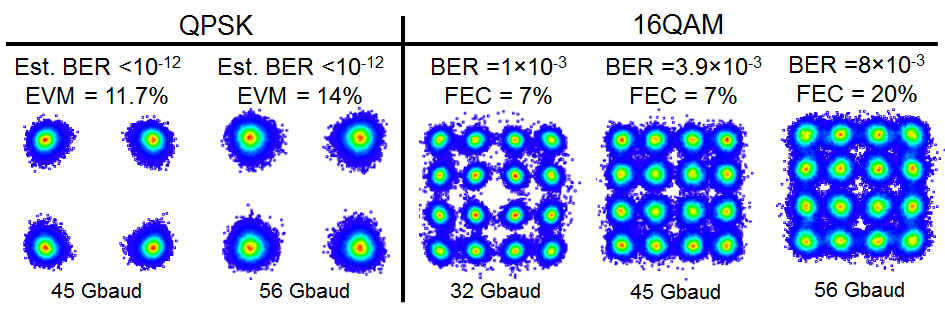
\includegraphics[width=0.8\textwidth]{caps/IQ_56gb}
  \caption{MCM IQ result summary. QPSK and 16QAM modulation was used to test the performance of the IQ modulator. Speeds of 32, 46 and 56 Gbaud were used and evaluated in error vector magnitude (EVM) QPSK and bit error probability (BER) for QPSK and 16QAM. Forward error correction (FEC) was considered for 16QAM format.}
  \label{fig:mcm-005-DTE-res}
\end{figure}

%% -------------------
%% | Example content |
%% -------------------

